\documentclass[dvipdfmx,twoside]{jsarticle}
\usepackage{amsmath,amssymb}
\usepackage{CJKutf8}
\usepackage{okumacro}
\usepackage{booktabs}
\usepackage{array}
\usepackage{xcolor}
\usepackage{colortbl}
\usepackage{tipa}
\usepackage{tikz}
\usepackage{fancybox}
\usepackage{wasysym}
\usepackage{pifont}
\usepackage{graphicx}
\usepackage{wrapfig}
\usepackage{geometry}
\geometry{margin=2cm}
\usepackage{fancyhdr}
\usepackage[utf8]{inputenc}
\usepackage{CJK}
\usetikzlibrary{positioning, intersections, calc, arrows.meta, math, through}
\usepackage{tcolorbox}
\tcbuselibrary{theorems,breakable}
\usepackage{enumerate}
% 设置页面样式
% \pagestyle{fancy}
% \fancyhf{}
% \renewcommand{\headrulewidth}{0pt}
% \fancyhead[RO]{数学–\thepage}
% \fancyhead[LE]{数学–\thepage}

% 重新定义 plain 样式
% \fancypagestyle{plain}{%
%   \fancyhf{}%
%   \renewcommand{\headrulewidth}{0pt}%
%   \fancyhead[RO]{数学-\thepage}%
%   \fancyhead[LE]{数学-\thepage}%
% }
\newtcbtheorem[]{reidai}{例題}
{fonttitle=\gtfamily\sffamily\bfseries\upshape\large,
colframe=black,colback=black!15!white,
rightrule=1pt,leftrule=1pt,bottomrule=2pt,
colbacktitle=black,theorem style=standard,breakable,arc=10pt}
{tha}
\newcommand{\kai}%解答
{\noindent
\begin{tikzpicture}[scale=0.2, baseline=2.8pt]
\draw (3.3,1) node{\large\textgt{解 答}};
\draw[thick, rounded corners=3pt,] (0,0)--(6.5,0)--(6.5,2.2)--(0,2.2)--cycle;
\end{tikzpicture}\;}
\newcommand{\shomei}%証明
{\noindent
\begin{tikzpicture}[scale=0.2, baseline=2.8pt]
\draw (3.3,1) node{\textgt{証 明}};
\draw[double,thick,rounded corners=3pt,] (0,0)--(6.5,0)--(6.5,2.2)--(0,2.2)--cycle;
\end{tikzpicture}\;}
%補足
\newcommand{\hosoku}{\noindent
\begin{tikzpicture}[scale=0.2, baseline=2.8pt]
\draw (6,1) node{\large\textgt{補足}};
\fill (0,1)--(1,0)--(2,1)--(1,2)--cycle;
\fill[gray] (1,1)--(2,0)--(3,1)--(2,2)--cycle;
\fill (2,1)--(3,0)--(4,1)--(3,2)--cycle;
\fill (10,1)--(11,0)--(12,1)--(11,2)--cycle;
\fill[gray] (9,1)--(10,0)--(11,1)--(10,2)--cycle;
\fill (8,1)--(9,0)--(10,1)--(9,2)--cycle;
\end{tikzpicture}\;}
%注意
\newcommand{\chui}{\noindent
\begin{tikzpicture}[scale=0.2, baseline=2.8pt]
\fill (0,0)--(6.5,0)--(6.5,2.2)--(0,2.2);
\draw (3.3,1) node[white]{\large\textgt{注意!}};
\draw[thick] (0,0)--(6.5,0)--(6.5,2.2)--(0,2.2)--cycle;
\end{tikzpicture}\;}
% 自定义A方框命令
\newcommand{\abb}[1]{%
\begin{tikzpicture}[baseline]
\node[draw=black, 
      rectangle, 
      minimum width=0.8cm, 
      minimum height=0.3cm, 
      fill=gray!25, 
      font=\bfseries,
      line width=1pt,
      inner sep=2pt,
      anchor=base] {#1};
\end{tikzpicture}%
}
\newcommand{\ab}[1]{%
\begin{tikzpicture}[baseline]
\node[draw=black, 
      rectangle, 
      minimum width=0.8cm, 
      minimum height=0.3cm, 
      font=\bfseries,
      line width=1pt,
      inner sep=2pt,
      anchor=base] {#1};
\end{tikzpicture}%
}

\newcommand{\maru}[1]{\tikz[baseline=-0.7ex]{
    \node[shape=circle,draw,inner sep=1pt,minimum size=5pt,anchor=center] {\footnotesize #1};}}
\definecolor{headercolor}{RGB}{220,220,220}
\definecolor{rowcolor1}{RGB}{245,245,245}
\definecolor{rowcolor2}{RGB}{255,255,255}

% \title{\vspace{-1.5cm} 2025年8月羚課文科数学月考 }
% \author{\textnosfal{Linc\ -\ 伊}}
\date{}
\begin{document}
\thispagestyle{empty}
\begin{CJK}{UTF8}{ipxm}  % 使用ipxm字体
  %月考表纸部分
\begin{center}

\vspace*{5cm}

% 学校logo

\includegraphics[width=5cm]{pics/1.jpg}

\vspace{2cm}

% 主标题
{\fontsize{24}{30}\selectfont\bfseries\sffamily
2025年8月\\
\vspace{1em}
羚課文科数学月考\\
\vspace{1em}
解答
}

\end{center}
%問題1の内容
\newpage
\section*{問題\textrm{I}}
\noindent
\textbf{問1}\qquad $ x^2+y^2=4 $のとき、 $ 2x+y $の最大値は$\ab{\textsf{A}}\sqrt{\ab{\textsf{B}}}$\\

2次関数$y = x^2 + 6x + 5$ のグラフを原点$(0,0)$に関して対称移動してできるグラフの方程式は\\
$$ y= \ab{\textsf{C}}\ x^2+\ab{\textsf{D}}\ x+\ab{\textsf{E}}$$
\\
\\

\kai\\

\noindent
(1)\quad $ x^2+y^2=4 $によって、 これは円の中心が$ (0,0) $、半径rが2の円である。 $ 2x+y $の最大値を $ k $とすると、 $ 2x+y=k\implies y=-2x+k\implies 2x+y-k=0$\ 
ここで、円の上に$2x+y$の最大値を得られる点$(x_0,y_0)$が存在する。よって、直線 $ 2x+y-k=0 $は円との関係は接する場合と交わる場合の2ケースだけである。したがって、
点と直線の距離の公式によって、円の中心座標を$2x+y-k=0$に代入すると $ d=\dfrac{|2\times 0+0-k|}{\sqrt{2^2+1^2}}\leq 2=r\ \implies |-k|\leq 2\sqrt{5}$となる。
$ |-k| = |k|$により、 $ |k|\leq 2\sqrt{5}\ \implies -2\sqrt{5}\leq k\leq 2\sqrt{5} $。以上より、 $ 2x+y $の最大値は $ 2\sqrt{5} $である。
\\

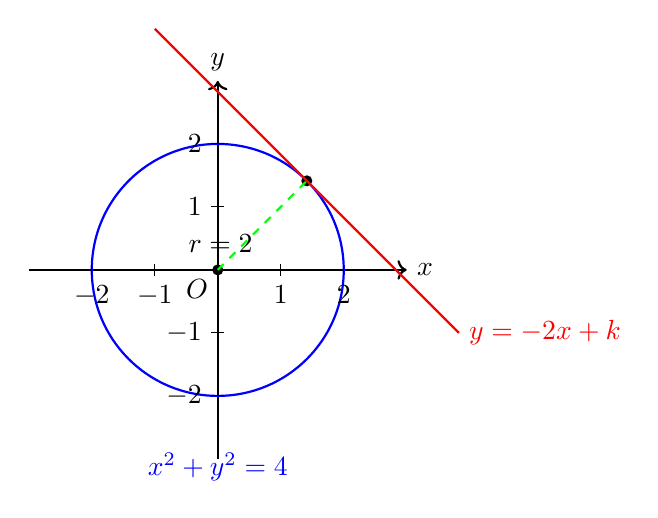
\begin{tikzpicture}[scale=0.8]
% 坐标轴
\draw[->, thick] (-3,0) -- (3,0) node[right] {$x$};
\draw[->, thick] (0,-3) -- (0,3) node[above] {$y$};

% 圆形 x^2 + y^2 = 4 (半径为2)
\draw[thick, blue] (0,0) circle (2);

% 坐标轴刻度
\foreach \i in {-2,-1,1,2} {
  \draw (\i,0.1) -- (\i,-0.1) node[below] {$\i$};
  \draw (0.1,\i) -- (-0.1,\i) node[left] {$\i$};
}

% 原点
\node[below left] at (0,0) {$O$};
\fill (0,0) circle (2.5pt);
\fill (1.414,1.414) circle (2.5pt);

% 相切直线 y = -x + 2√2 (斜率为-1)
\draw[thick, red] (-1,3.828) -- (3.828,-1) node[right] {$y = -2x + k$};

% 从圆心到直线的垂直距离
\draw[dashed, green, thick] (0,0) -- ({sqrt(2)},{sqrt(2)});



% 距离标注
\node[below left] at ({sqrt(2)/2},{sqrt(2)/2}) {$r=2$};

% 标题
\node[above] at (0,-3.5) {\color{blue}{$x^2 + y^2 = 4$}};
\end{tikzpicture}
\\

\noindent
(2)\quad 原点に関して対称移動: $x$を$-x$に、$y$を$-y$に変える。したがって、$ y=-f(-x)\implies y=-x^2+6x-5 $\\
すなわち\textcolor{red}{$y=-x^2+6x-5$}\\
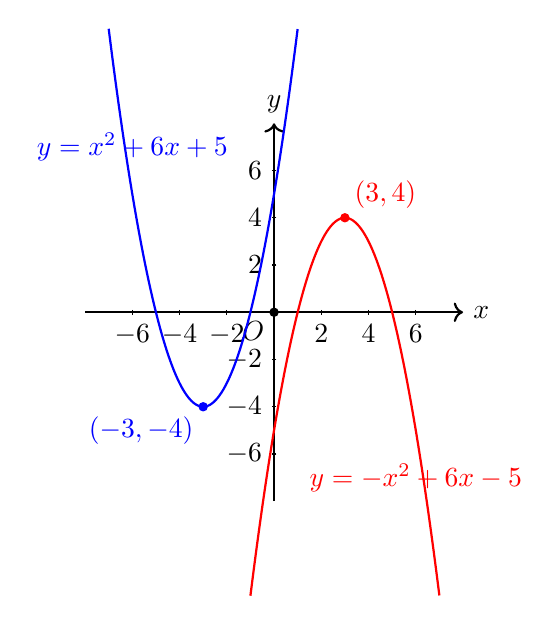
\begin{tikzpicture}[scale=0.3]
% 坐标轴
\draw[->, thick] (-8,0) -- (8,0) node[right] {$x$};
\draw[->, thick] (0,-8) -- (0,8) node[above] {$y$};

% 坐标轴刻度
\foreach \i in {-6,-4,-2,2,4,6} {
    \draw (\i,0.1) -- (\i,-0.1) node[below] {$\i$};
    \draw (0.1,\i) -- (-0.1,\i) node[left] {$\i$};
}

% 原点
\node[below left] at (0,0) {$O$};
\fill[black] (0,0) circle (0.2);

% 原函数 y = x^2 + 6x + 5
\draw[thick, blue, domain=-7:1, samples=100] 
    plot (\x, {\x*\x + 6*\x + 5});

% 对称移动后的函数 y = -x^2 - 6x - 5
\draw[thick, red, domain=-1:7, samples=100] 
    plot (\x, {-\x*\x + 6*\x - 5});

% 顶点
\fill[blue] (-3,-4) circle (0.2) node[below left] {$(-3,-4)$};
\fill[red] (3,4) circle (0.2) node[above right] {$(3,4)$};


% 函数标签
\node[blue, above] at (-6,6) {$y = x^2 + 6x + 5$};
\node[red, below] at (6,-6) {$y = -x^2 + 6x - 5$};
\end{tikzpicture}
\newpage
\noindent
\textbf{問2}\qquad $3a + 1$ が $a^2 + 5$ の約数となるような自然数 $a$ を求めよう。

\vspace{2em}

$3a + 1 = b$ とする。このとき

\vspace{1em}

\begin{center}
$a^2 + 5 = \dfrac{b^2 - \ab{\textsf{F}}\ b + \ab{\textsf{GH}}}{\ab{\textsf{I}}}$ \hspace{2em} $\cdots\cdots$ \maru{1}
\end{center}

\vspace{1em}

である。また、$b$ は $a^2 + 5$ の約数であるから、$a^2 + 5$ はある自然数 $c$ を用いて

\vspace{1em}

\begin{center}
$a^2 + 5 = bc$ \hspace{2em} $\cdots\cdots$ \maru{2}
\end{center}

\vspace{1em}
と表される。\maru{1}、\maru{2} から

\vspace{1em}

\begin{center}
$b\left(\ab{\textsf{J}}\ c - b + \ab{\textsf{K}}\right) = \ab{\textsf{LM}}$
\end{center}

\vspace{1em}

を得る。したがって、$b$ は \abb{\textsf{LM}} の約数である。この中で、$a$ が自然数となるのは $b =$ \ab{\textsf{NO}}

\vspace{1em}

である。したがって、$a = \ab{\textsf{PQ}}$ である。
\\
\\

\kai\\

\noindent
(1)\quad $3a + 1 = b$とすると、$a=\dfrac{b-1}{3}$となって、$a$を$a^2+5$に代入すると、$a^2 + 5 = \dfrac{(b-1)^2}{9} + 5 = \dfrac{b^2 - 2b + 1 + 45}{9} = \dfrac{b^2 - {\color{red}{2} }b + \color{red}{46}}{\color{red}{9}}$となる。\\

\noindent
(2)\quad \maru{1}と\maru{2}の式から、 $ a^2+5=bc=\dfrac{b^2 - 2b + 46}{9}\ \implies\ 9bc-b^2+2b=46\ \implies\ b({\color{red}{9}}c-b+{\color{red}{2}})=\color{red}{46}$。\\

\noindent
(3)\quad $b$は$46$の約数である。したがって、$b$は$1,2,23,46$のいずれかである($46=46\times 1=2\times 23\times =1$)。$a$が自然数と$b=3a+1$の条件によって、 $b\geq 4$となる。したがって、$b=23$の場合は、$a=\dfrac{b-1}{3}=\dfrac{22}{3}$であり、$a$の条件を満たさない。$b=46$の場合は、$ a=\dfrac{b-1}{3}=\dfrac{45}{3}=15$であり、$a$の条件を満たす。したがって、$b={\color{red}{46}},a=\color{red}{15}$が求める答えである。\\

%問題2の内容
\newpage
\section*{問題\textrm{II}}
\noindent
\textbf{問1}\qquad 大きさの異なる4枚のカードがある。これらのカードに赤、黒、青、黄の色を塗る。ただし、\\
\hspace*{1em}どのカードにも1つの色のみを使い、また同じ色のカードが2枚以上あってもよいものとする。

\vspace{1em}

(1) \hspace{1em} 全部で \ab{\textsf{ABC}} 通りの塗り方がある。

\vspace{1em}

(2) \hspace{1em} 全部の色を使う塗り方は \ab{\textsf{DE}} 通りある。

\vspace{1em}

(3) \hspace{1em} 2枚は赤で、1枚が黒、1枚が青となるような塗り方は \ab{\textsf{FJ}} 通りある。

\vspace{1em}

(4) \hspace{1em} 3つの色を使う塗り方は \ab{\textsf{GHI}}  通りある。

\vspace{1em}

(5) \hspace{1em} 2つの色を使う塗り方は \ab{\textsf{JK}} 通りある。
\\
\\

\kai\\ 

\noindent
(1)\quad 各カードに4色のうち1色を塗るので、4枚のカードに対しては $4^4=256$ 通りの塗り方がある。したがって、全部で $\color{red}{256}$通りの塗り方がある。\\
\vspace{1em}

\begin{tikzpicture}
% カード1: 対角線で4等分
\begin{scope}[shift={(0,0)}]
\draw[thick] (0,0) rectangle (0.8,1.2);
\fill[red!40] (0,0.6) rectangle (0.4,1.2);
\fill[blue!40] (0.4,0.6) rectangle (0.8,1.2);
\fill[yellow!40] (0,0) rectangle (0.4,0.6);
\fill[black!50] (0.4,0) rectangle (0.8,0.6);
\node at (0.4,0.6) {\small A};
\node at (0.4,1.5) {\small $4$通り};
\end{scope}

% カード2: 縦横分割
\begin{scope}[shift={(1.2,0)}]
\draw[thick] (0,0) rectangle (0.8,1.2);
\fill[red!40] (0,0.6) rectangle (0.4,1.2);
\fill[blue!40] (0.4,0.6) rectangle (0.8,1.2);
\fill[yellow!40] (0,0) rectangle (0.4,0.6);
\fill[black!50] (0.4,0) rectangle (0.8,0.6);
\node at (0.4,0.6) {\small B};
\node at (0.4,1.5) {\small $4$通り};
\end{scope}

% カード3: 扇形分割
\begin{scope}[shift={(2.4,0)}]
\draw[thick] (0,0) rectangle (0.8,1.2);
\fill[red!40] (0,0.6) rectangle (0.4,1.2);
\fill[blue!40] (0.4,0.6) rectangle (0.8,1.2);
\fill[yellow!40] (0,0) rectangle (0.4,0.6);
\fill[black!50] (0.4,0) rectangle (0.8,0.6);
\node at (0.4,0.6) {\small C};
\node at (0.4,1.5) {\small $4$通り};
\end{scope}

% カード4: 水平分割
\begin{scope}[shift={(3.6,0)}]
\draw[thick] (0,0) rectangle (0.8,1.2);
\fill[red!40] (0,0.6) rectangle (0.4,1.2);
\fill[blue!40] (0.4,0.6) rectangle (0.8,1.2);
\fill[yellow!40] (0,0) rectangle (0.4,0.6);
\fill[black!50] (0.4,0) rectangle (0.8,0.6);
\node at (0.4,0.6) {\small D};
\node at (0.4,1.5) {\small $4$通り};
\node at (2,0.7) {\Large $\implies 4^4$通り};
\end{scope}
\end{tikzpicture}
\\

\noindent
(2)\quad 4色全てが最低1回は使われる塗り分けである。カードをA,B,C,Dとすると、最初Aは4択を選べられ、まず赤を塗るとする。次のBは赤抜きの3色しか選べられないので、3通りがあって、黒を塗るとする。
Cは赤と黒抜きの2色しか選べられないので、2通りがあって、ここで青を塗るとする。最後の黄色をDに塗るしかないので、合計で$4!=4\times 3\times 2\times 1 = \color{red}{24}$通りがある。
\vspace{1em}

\begin{tikzpicture}
\node[draw, rectangle, fill=red!40, minimum width=0.8cm, minimum height=1.2cm] (A) at (0,0) {A};
\node[draw, rectangle, fill=black!40, minimum width=0.8cm, minimum height=1.2cm] (B) at (1.2,0) {B};
\node[draw, rectangle, fill=blue!30, minimum width=0.8cm, minimum height=1.2cm] (C) at (2.4,0) {C};
\node[draw, rectangle, fill=yellow!40, minimum width=0.8cm, minimum height=1.2cm] (D) at (3.6,0) {D};
\node at (0,-0.9) {4通り};
\node at (1.2,-0.9) {3通り};
\node at (2.4,-0.9) {2通り};
\node at (3.6,-0.9) {1通り};
\node at (5.2,0) {\Large $ \implies 4! $通り};
\end{tikzpicture}
\\

\noindent
(3)\quad 最初は4枚のカードから2枚を選んで赤を塗ると、 $ {}_4\mathrm{C}_2=\dfrac{4!}{2!2!}=6 $通りがある。次に、残りの2枚カードから1枚を選んで黒を塗ると、$ {}_2\mathrm{C}_1=2 $通りがある。最後の1枚カードは青を塗ると、1通りがある。
したがって、合計で$6\times 2\times 1 = \color{red}{12}$通りである。
\vspace{1em}

\begin{tikzpicture}
\node[draw, rectangle, fill=red!40, minimum width=0.8cm, minimum height=1.2cm] (A) at (0,0) {A};
\node[draw, rectangle, fill=red!40, minimum width=0.8cm, minimum height=1.2cm] (B) at (1.2,0) {B};
\node[draw, rectangle, fill=black!40, minimum width=0.8cm, minimum height=1.2cm] (C) at (2.4,0) {C};
\node[draw, rectangle, fill=blue!30, minimum width=0.8cm, minimum height=1.2cm] (D) at (3.6,0) {D};
\node at (0.6,-0.8) {$\underbrace{\phantom{A\quad B}}_{{}_4\mathrm{C}_2=6 通り}$};
\node at (2.4,-0.9) {2通り};
\node at (3.6,-0.9) {1通り};
\node at (6.6,0) {\Large $ \implies 6\times 2\times 1 = 12 $通り};
\end{tikzpicture}
\\

\noindent
(4)\quad 最初4色から3色を選んで、 $ {}_4\mathrm{C}_3=4 $通りがある。次に、選んだ3色の中で1つの色が2回使われた選び方は $ {}_3\mathrm{C}_1  = 3$通りがある。
次の塗り方は(3)と同じであって、合計で $ 4\times 3\times 12 =\color{red}{144} $通りである。  
\\

\noindent
(5)\quad 1つの色を使う塗り方は4色がある。したがって、2つの色を使う塗り方は $ 256-(24+144+4)=\color{red}{84} $通り。
\newpage
\noindent
\textbf{問2}\qquad 2つの放物線\\
\\
$\ell: \quad y = ax^2 + 2bx + c$\\
$m: \quad y = (a+1)x^2 + 2(b+2)x + c + 3$\\
\\
\begin{wrapfigure}{r}{0.4\textwidth}
\vspace{-8em}
\begin{tikzpicture}[scale=0.8]
\draw[->] (-3,0) -- (3,0) node[right] {$x$};
\draw[->] (0,-2) -- (0,3) node[above] {$y$};
\node[below left] at (0,0) {O};
\node[above left] at (-2,0) {A};
\node[below left] at (-1.5,-1.5) {B};
\node[above right] at (-1,0) {C};
\node[below right] at (1,0) {D};
\fill (-2,0) circle (2pt);
\fill (-1.5,-1.5) circle (2pt);
\fill (-1,0) circle (2pt);
\fill (1,0) circle (2pt);
\fill (0,0) circle (2pt);
\end{tikzpicture}
\end{wrapfigure}

\noindent
を考える。点 A, B, C, D が右図のような位置関係に
\noindent
あるとする。このとき,この 2 つの放物線のうち,
\noindent
一方は,3 点 A, B, C を通り,もう一方は,3 点 B,
\noindent
C, D を通るとする。

\vspace{1em}
\noindent
(1)\quad 3 点 A, B, C を通る放物線は \ab{\textsf{L}} である。ただし、\\
\ab{\textsf{L}} には,次の\maru{0}か\maru{1}のどちらか適するものを選びなさい。

\vspace{0.5em}

\begin{center}
\begin{tabular}{cc}
\maru{0} & 放物線 $\ell$ \\
\maru{1} & 放物線 $m$
\end{tabular}
\end{center}

\vspace{1em}
\noindent
(2)\quad 2 つの放物線 $\ell, m$ は,どちらも 2 点 B, C を通るので,点 B, C の座標は,2 次方程式

\[x^2 + \ab{\textsf{M}}\ x + \ab{\textsf{N} }= 0\]

の解である。よって,点 B の $x$ 座標は \ab{\textsf{OP}},点 C の $x$ 座標は \ab{\textsf{QR}} である。

\vspace{1em}
\noindent
(3)\quad 特に,AB = BC, CO = OD のとき,$a, b, c$ の値を求めよう。\\

\quad 2 点 C, D は $y$ 軸に関して対称であるから,$b = \ab{\textsf{S}}$ である。また,AB = BC より,\\

直線 $x = \ab{\textsf{TU}}$ が\ \abb{\textsf{L}}\ の軸である。したがって,$a = -\ \displaystyle\dfrac{\ab{\textsf{V}}}{\ab{\textsf{W}}}$ である。よって,\\


$c = \dfrac{\ab{\textsf{X}}}{\ab{\textsf{Y}}}$ である。
\\
\\

\kai\\

\noindent
(1)\quad 問題の条件から、 $\ell$と$m$の放物線の傾きの正負は異なる。よって、 $ a\leq 0\leq a+1 $が成り立つ。したがって、3点$A,B,C$を通る放物線は{\color{red}\maru{1}}の放物線$m$である。\\

\noindent
(2)\quad 3点$A,B,C$を通る放物線は$m$である。3点$B,C,D$を通る放物線は$\ell$である。したがって、$m$と$\ell$の方程式は点$B,C$を通るので、$y=ax^2+bx+c=(a+1)x^2+2(b+2)x+c+3\ \implies\ x^2+{\color{red}4}x+{\color{red}3}=0$ 。
この方程式の解は、点$B,C$の$x$座標である。$x^2+4x+3=0\ \implies\ (x+4)(x+3)=0$\ したがって、点$B$の$x$座標は$\color{red}-3$,\ 点$C$の$x$座標は$\color{red}-1$となる。\\

\noindent
(3)\quad 点$C,D$は$y$軸に関して対称であるから、$\ell$の頂点$x$座標は$-\dfrac{2b}{2a}=-\dfrac{b}{a}=0$である。したがって、$b=\color{red}{0}$となる。$AB=BC$より、直線 $x=\color{red}{-3}$ が$m$の軸である。したがって、$m$の放物線の頂点$x$座標により、$-\dfrac{2(b+2)}{2(a+1)}=-\dfrac{0+2}{a+1}=-3 \implies a=-\color{red}{\dfrac{1}{3}}$である。よって、$c=\dfrac{1}{2}$である。点$C:(-1,0)$を$\ell$の方程式に代入すると、 $a\times (-1)^2+2\times 0\times x+c=0 \implies -\dfrac{1}{3}+c=0 \implies c=\color{red}{\dfrac{1}{3}}$である。

\end{CJK}
\end{document}


